\chapter{Techniki harcerskie}
Z powodu ograniczonego miejsca, ten rozdział jest bardzo ogólnikowy.
\section{Terenoznawstwo}

Orientacja w terenie jest jedną z ważniejszych umiejętności jaką powinien posiadać każdy harcerz. Orientowanie się w terenie oprócz umiejętności zorientowania mapy ułatwia również obserwacja zjawisk przyrody. 
\paragraph{Sposoby orientacji w terenie}
\begin{description}[noitemsep,nolistsep] 

\item[Według położenia słońca] --- polega na ustawieniu się w słoneczny dzień w południe tyłem do słońca i zorientowaniu wg zasady że nasz cień pokazuje południe
\item[Według słońca i zegarka] --- jest to dość dokładna metoda ---- małą wskazówkę zegarka kierujemy ku słońcu. 
Teraz kąt między wskazówką, a cyfrą 12 dzielimy na połowę. Linia podziału wskazuje kierunek południowy (o 12:00). 
Pamiętać trzeba, że przed południem bierzemy pod uwagę kąt między małą wskazówką, a godz. 12. Po południu kąt między linią na godzinę 12, a małą wskazówkę
\item[Według gwiazdy polarnej] --- znajdujemy najpierw Wielki Wóz, a następnie przeprowadzamy przez dwie skrajne gwiazdy prostej, na której okładamy 5-krotną odległość między tymi gwiazdami. 
Na końcu tego odcinka znajduje się Gwiazda polarna wyznaczająca północ.
\item[W starych kościołach] ołtarze skierowane są w kierunku wschodnim.

\end{description}
\paragraph{Skala mapy}

Skala mapy informuje nas ile razy dana mapa została pomniejszona. Jak obliczyć jaka odległość na mapie odpowiada jakiej odległości w rzeczywistości? Jest to szalenie proste wystarczy z danej skali, np. 1:100000 skreślić 5 ostatnich cyfr. Wyjdzie nam wtedy, że 1 cm. na mapie odpowiada 1 km. w rzeczywistości. Szczegółowe mapy w Poznaniu można kupić na ul. Hawelańskiej 10 w Wojewódzkim Ośrodku Dokumentacji i Kartografii. Świetne mapy są dostępne także na stronie projektu http://geoportal.gov.pl

\paragraph{Mierzenie w terenie}

W terenie znajdują się różne rzeczy, których normalny śmiertelnik nie jest w stanie zmierzyć. No ale jako ze my jesteśmy harcerzami i dajemy sobie radę w wielu sytuacjach, to i w tym wypadku nie będzie to dla nas problem.

Pomiar szerokości rzeki - wbijamy krótką tyczkę na brzegu rzeki, i oddalamy się od niej z laską skautową na taka odległość, żeby z końca laski widzieć równocześnie koniec tyczki i krawędź drugiego brzegu.

Teraz za pomocą wzoru obliczamy szerokość rzeki: $AB= (DE x BD)/EF$
\begin{figure}[h]
\begin{center}
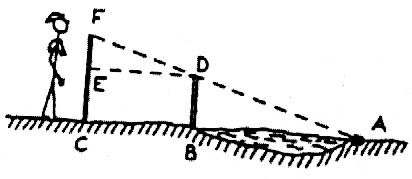
\includegraphics[width=0.7\textwidth]{grafiki/rzeka.png}
\end{center}
\end{figure}

2) Pomiar wysokości drzewa - sposób 1. 
Jeden z harcerzy zaznacza na lasce wyraźnie swoją wysokość od stóp do poziomu oczu, potem kładzie się na ziemi na wznak w odległości od podstawy drzewa przypuszczalnie równej wysokości drzewa. 
Drugi trzyma laskę pionowo przy jego stopach. 
Leżący przesuwa się na ziemi tak długo, aż znajdzie punkt, z którego przez miejsce zaznaczone na lasce zobaczy wierzchołek drzewa. 
Zmierzona ilość kroków od oka leżącego do podstawy drzewa na metry jest wysokością drzewa.
\begin{figure}[h]
\begin{center}
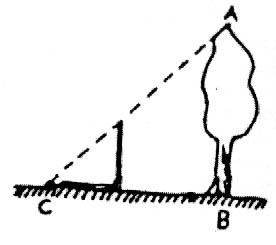
\includegraphics[width=0.3\textwidth]{grafiki/pomiardrzewa.png}
\end{center}
\end{figure}

3) Pomiar wysokości drzewa - sposób 2. Jeden z harcerzy staje pod drzewem. 
Drugi bierze kijek i stając w pewnej odległości przy wyciągniętej ręce z kijkiem zaznacza na nim wysokość harcerza. 
Następnie przy tej samej odległości i takim samym wyciągnięciu ręki mierzy kijkiem wysokość drzewa. 
Otrzymaną wysokość drzewa dzieli przez wysokość harcerza. 
Otrzymaną liczbę trzeba już tylko pomnożyć prze rzeczywisty wzrost harcerza.

\section{Łączność}
\begin{wrapfigure}{l}{3cm}
  \begin{center}
    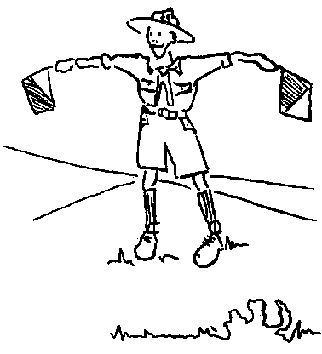
\includegraphics[width=3cm]{grafiki/lacznik.png}
  \end{center}
\end{wrapfigure} Łączność To bardzo rozległa dziedzina. 
Nie jest to wbrew pozorom tylko alfabet Morse’a i kilka innych szyfrów. 
Łączność to komunikacja międzyludzka za pomocą różnego rodzaju urządzeń i szyfrów. 
Do łączności zaliczają się więc m.in. : wysyłanie e-maili, rozmowa telefoniczna, łączność krótkofalarska, rozmowa za pomocą alfabetu Morse’a czy przekazywanie sobie nawzajem zaszyfrowanych wiadomości. 
	
\textbf{Alfabet Morse’a}
W 1837 roku niejaki Samuel Finley Breese Morse wynalazł telegraf elektromagnetyczny, a w 1840 stworzył dla niego specjalny alfabet telegraficzny zwany właśnie alfabetem Morse’a. 
Dzięki temu można było na duże odległości przekazywać sobie w krótkim czasie wiadomości, co było wcześniej niemożliwe. 
Obecnie alfabet Morse’a oprócz tego, że stosowany jest przez harcerzy, to wykorzystują go np. krótkofalowcy w łącznościach długodystansowych.

Alfabet ten składa się z kropek i kresek, które ułożone w odpowiedniej kolejności tworzą daną literę alfabetu. 
Żeby łatwiej było szyfrować i odczytywać wiadomości istnieje taka zasada: do każdej litery alfabetu przyporządkowywany jest odpowiedni wyraz, który dzielimy na sylaby. 
Jeśli w danej sylabie znajduje się „o” to piszemy kreskę, w przeciwnym razie kropkę.


\section{Szyfry}

Szyfr ułamkowy:
Jest to prosty szyfr. Alfabet dzielimy na poszczególne grupy i każdej takiej grupie przyporządkowujemy kolejno mianownik: 1, 2, 3, 4, 5. Potem przy zapisie w liczniku piszemy numer porządkowy danej litery, a mianownik przepisujemy. Litery i wyrazy można łączyć dowolnymi znakami matematycznymi\ldots
\begin{figure}[h]
\begin{center}
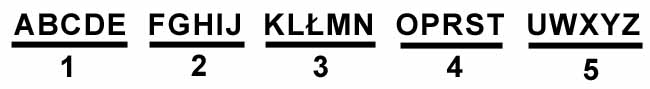
\includegraphics[width=0.9\textwidth]{grafiki/ulamkowy1.png}
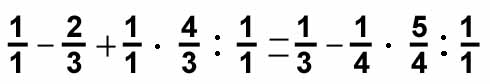
\includegraphics[width=0.9\textwidth]{grafiki/ulamkowy2.png}
\end{center}
\end{figure}



Szyfr ramowy/czekoladka:
\begin{figure}[h]
\begin{center}
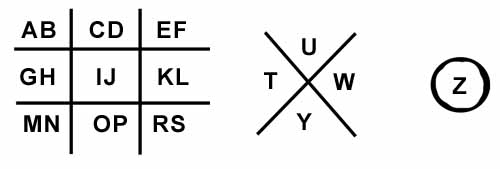
\includegraphics[width=0.9\textwidth]{grafiki/czekoladka.png}
\end{center}
\end{figure}

\paragraph{Pozostałe szyfry:}
Bardzo popularne szyfry takie jak GA-DE-RY PO-LU-KI, dzielimy go na sylaby, a następnie każdą literę, którą mamy zamienić zamieniamy na tę obok. Jeśli w szyfrze nie ma takiej litery, to ją normalnie przepisujemy. Istnieją też inne szyfry działające na tej samej zasadzie, takie jak: KONIEC MATURY, DALEKO TURYNI, KACE MINUTOWY, czy POLITYKA RENU.

\paragraph{Stwórz szyfr zastępu} --- tak by nikt inny nie mógł odczytywać Waszych wiadomości.




